\chapter{État de l'art} % Main chapter title

\label{Chapitre2} % For referencing the chapter elsewhere, use \ref{Chapter1} 

\lhead{Chapitre 2. \emph{État de l'art}} % This is for the header on each page - perhaps a shortened title
Plusieurs travaux par rapport à la gestion des variations ont été déjà effectués. Comme par exemple les travaux de \cite{sacl}, \cite{alm}, \cite{kabaaj}, \cite{gc}, etc. Ce qui veut dire que des solutions ont déjà été proposées. Alors dans ce chapitre, nous allons parler de la modélisation des procédés ainsi que les solutions qui traitent les variations au cours de l'évolution du projet.\\
\section{Modélisation des procédés}
Le développement d'un logiciel suit au moins ce qu'on appelle un procédé.  Ce procédé définit toutes les étapes nécessaires pour sortir un produit réussi. Aujourd'hui, la qualité de la modélisation des procédés occupe une place importante dans la réalisation d'un logiciel car la réussite du produit en dépend \cite{wsh73} \cite{abgm}.\\
On peut alors définir un procédé logiciel comme un ensemble d'activités aussi techniques qu'administratives pour développer et maintenir un produit logiciel \cite{jl}.\\
\subsection{Modèle de procédé}
Le modèle de procédé est une abstraction du procédé réel. Il décrit les éléments de procédé et les relations entre eux. Il y a plusieurs discussions par rapport aux éléments à décrire dans les modèles de procédés. Malgré cette divergence, il existe des points communs qui qui ont été recueillis dans plusieurs études \cite{jl} \cite{abgm} \cite{ac} \cite{fin}.\\
Han Nhi Tran \cite{hnt10} propose une classification de ces éléments en deux catégories.
\begin{enumerate}
\item Éléments primaires\\
Ils représentent le cœur des procédés. Ces éléments ne tiennent pas compte des aspects de planification et d'exécution de procédé. Ce sont:
\begin{itemize}
\item[\tiny{$\blacksquare$}] les activités: L'ensemble des actions effectuées par les rôles pour accomplir un objectif dans le développement \cite{ml11}.
\item[\tiny{$\blacksquare$}] les produits: ce sont des artéfacts \footnote{ les artéfacts sont des produits créés ou modifiés pendant un procédé} utilisés ou élaborés par les activités durant le développement.
\item[\tiny{$\blacksquare$}] les rôles: un rôle décrit un ensemble de responsabilités, droits et compétences d'un agent dans le contexte des activités ou il intervient\cite{ml11}. 
\end{itemize}
\item Éléments secondaires\\
Ce sont des éléments fournissant des informations supplémentaires pour la mise en œuvre d'un procédé. Ces éléments sont: 
\begin{itemize}
\item[\tiny{$\blacksquare$}] les agents: un agent est celui qui exécute le procédé \footnote{ tous les éléments impliquées dans le développement et la maintenance d'un produit ou service, c'est à dire artefacts, support de production (outils), activités agents}. Il peut être un humain ou un outil logiciel. Un agent n'est pas un rôle, mais il est caractérisé par les propriétés de son ou ses rôle(s) \cite{ml11} 
\item[\tiny{$\blacksquare$}] les ressources: ce sont des éléments facilitant l'exécution d'une activité \cite{hnt10}
\item[\tiny{$\blacksquare$}] les informations qualitatives : ce sont des informations permettant d'évaluer la performance et la qualité de procédés. Ces informations peuvent être des résultats de révision ou test, des métriques etc.\cite{hnt10}
\item[\tiny{$\blacksquare$}] les informations organisationnelles: ce sont des informations qui facilitent l'exécution d'un procédé pour un projet spécifique
\end{itemize}
\end{enumerate}
\clearpage
La figure \ref{mcp} est un modèle conceptuelle de procédés, elle montre les différentes relations existantes entre les éléments de procédés.
\begin{figure}[h]
\centering
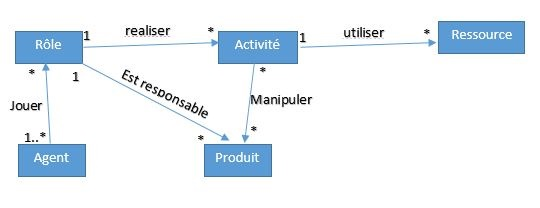
\includegraphics[width=13cm]{modeleProcede.jpg}
\caption{\label{mcp}Modèle conceptuel de procédés \cite{hnt10}}
\end{figure}

\subsection{Langage de modélisation de procédés }
Pour décrire un modèle de procédé, nous avons besoin de langage, ce langage est appelé « Langage de modélisation de procédés » ou \textit{"Process Modeling Language (PML)"} \cite{ac} \cite{rc} \cite{sl} ou encore \textit{"Software Process Modeling Language (SPML)"} \cite{alm}. \\
Ils existent plusieurs langages de modélisation de procédés logiciel, mais d'après les études de \cite{abgm} \cite{vra} \cite{jab}, les propriétés les plus importantes attendues d'un PML sont:
\begin{enumerate}
\item Formalisation: cette propriété représente le degré de formalisation (définition syntaxique) et de la sémantique du PML. Il existe trois degrés de formalisation: formel \footnote{un langage formel est un langage dont la sémantique et la syntaxe sont bien définis}, informel \footnote{langage non défini avec des concepts, une syntaxe et une sémantique}, semi-formel\footnote{langage dont la syntaxe est précise mais la sémantique non}.
\item Expressivité: cette catégorie reflète la capacité du PML à représenter tous les éléments du procédé.
\item Compréhensibilité: elle peut être textuel ou graphique, cette propriété reflète le degré de facilité à comprendre le modèle décrit à travers la notation du PML.
\item Abstraction et modularité: elles représentent la capacité du PML à proposer des mécanismes d'abstraction et d'agrégation afin de structurer les procédés pour une facilitation de la réutilisation.
\item Exécutabilité: c'est la capacité du PML à représenter des modèles exécutables (opérationnels). 
\item Évolutivité: c'est la capacité de supporter l'évolution de modèles de procédé. 
\item Multi-vue: la capacité à supporter les modèles d'activités, produits, rôles, ressources 
\end{enumerate}
En étudiant les PMLs, on s'aperçoit qu'ils peuvent utilisés différentes approches afin de mieux répondre aux besoins de la phase. Nous n'allons pas citer toutes les approches existantes, mais nous présenterons quelques une des plus connues. Parmi ces approches nous avons:
\begin{itemize}
\item approche procédurale: proposée dans \cite{lo}, l'approche procédurale permet de représenter le modèle de procédé sous la forme d'un programme. Ce programme décrit de manière détaillé comment le procédé logiciel doit être réalisé.
\item approche déclarative: cette approche utilise des déclarations logiques (règles) pour décrire les procédés logiciels. Ceux-ci sont décrits en termes de résultats attendus par l'utilisateur sans détailler la manière dont ces résultats sont obtenus \cite{lgw}.
\item approche fonctionnelle: l'approche fonctionnelle définit le procédé logiciel à travers un ensemble de fonctions mathématiques. Chaque fonction est décrite en termes de relations entre les données d'entrée et les données de sortie. 
\item approche basée sur les réseaux de pétri: cette approche permet de décrire le procédé logiciel à travers un réseau de pétri\footnote{un réseau de pétri est un moyen de: - modélisation du comportement des systèmes dynamiques à évènements discrets; - description des relations existantes entre des conditions et des évènements}.
\item approche basée sur UML: cette approche utilise des diagrammes UML pour représenter les concepts du procédé et renforce la sémantique de ces diagrammes avec un langage formel pour rendre les modèles de procédé à la fois compréhensifs et exécutables. 
Plusieurs approches ont été développées avec cette perspective, notamment le standard de l'OMG (société Américaine créée en 1989, il est à la base des standards UML, MOF \textit{"Meta-Oject Facility"}, CORBA \textit{"Common Object Request Broker Architecture"}, CWM \textit{"Common Warehouse Metamodel"}) \textit{"Object Management Group"} SPEM.
\subsubsection*{\textit{Software Process Engineering Metamodel} (SPEM)}
le méta-modèle d'ingénierie des procédés logiciels est à la fois un méta-modèle (c'est un langage de modélisation permettant d'exprimer les concepts conforme au MOF) et un profil UML (il est basé sur du UML). Le leitmotiv d'un SPEM est qu'un procédé de développement logiciel est une collaboration entre des rôles exécutant des actives sur des produits. \\
Il existe deux versions de SPEM: \textbf{SPEM 1.1} et \textbf{SPEM 2.0}.
\begin{itemize}
\item[\tiny{$\blacktriangleright$}] SPEM 1.1: première version de SPEM, adopté en janvier 2005 \cite{omg1}, il était composé de deux groupes : le \textit{SPEM foundation} qui fournit les concepts de base pour définir le méta-model SPEM et le \textit{SPEM-Extension} qui décrit le concept de base pur décrire les processus logiciels. 
\item[\tiny{$\blacktriangleright$}] SPEM 2.0: cette version est la plus récente de SPEM. Le SPEM 2.0 est structuré en sept paquetages \cite{omg2} comme le montre la figure \ref{sspem}.
\clearpage
\begin{figure}[h]
\centering
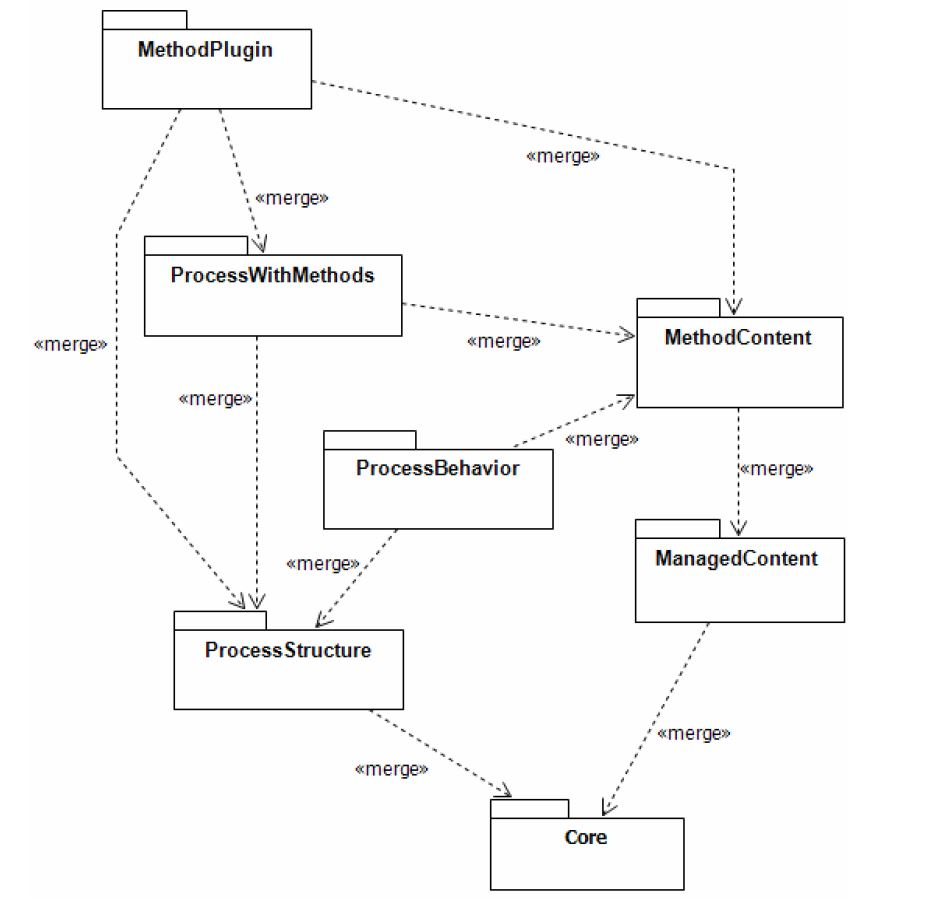
\includegraphics[width=13cm]{strucspem.jpg}
\caption{\label{sspem}Structure du SPEM 2.0 \cite{omg2}}
\end{figure}
\begin{itemize}
\item[\tiny{$\blacksquare$}] \textbf{ \textit{MethodPlugin}}: dans ce paquetage, seront gérés les librairies et les référentiels méthodologiques.
\item[\tiny{$\blacksquare$}] \textbf{ \textit{ProcessWithMethods}}: ce paquetage permet de définir ou de redéfinir les éléments pour intégrer les processus définis avec les concepts du paquetage \textit{ProcessStructure}, selon les contenus définis avec les concepts du paquetage \textit{MethodContent} ;
\item[\tiny{$\blacksquare$}] \textbf{ \textit{MethodContent}}: ce paquetage fournit les concepts pour que les utilisateurs puissent spécifier le contenu des méthodes comme les rôles \textit{(Roles)}, les tâches \textit{(Tasks)}, etc.; 
\item[\tiny{$\blacksquare$}] \textbf{ \textit{ProcessBehavior}}: il offre la possibilité de lier un élément de procédé SPEM 2.0 avec un comportement externe comme un modèle BPMN \textit{(Business Process Modeling Notation)} ou un modèle UML 2.
\item[\tiny{$\blacksquare$}] \textbf{ \textit{ManagedContent}}: ce paquetage fournit les concepts pour gérer les descriptions textuelles des éléments de procédés.
\item[\tiny{$\blacksquare$}] \textbf{ \textit{ProcessStructure}}: ce paquetage définit la base pour représenter tous les modèles de procédés.
\item[\tiny{$\blacksquare$}] \textbf{ \textit{Core}}: il contient les éléments de base (classes et abstractions) utilisés dans les autres paquetages. 
\end{itemize}
\end{itemize} 
\end{itemize}
Après la présentation des modèles de procédés et des langages de modélisation, nous allons passer aux environnements de génie logiciel centrés procédé.
\section{Process-Centered Software Engineering Environments (PSEE)}
Un PSEE est un environnement de travail permettant de fournir divers services aux développeurs par l'exécution des modèles de processus. Ces services sont multiples, parmi lesquels nous avons : l'aide aux développeurs logiciel, l'automatisation de certaines tâches, l'invocation et le contrôle des outils de développement logiciel, le contrôle de l'application des règles obligatoires, etc.\cite{vra}. \\
La figure \ref{rolepsee} résume le rôle d'un PSEE dans le processus de développement d'un logiciel.
\begin{figure}[h]
\centering
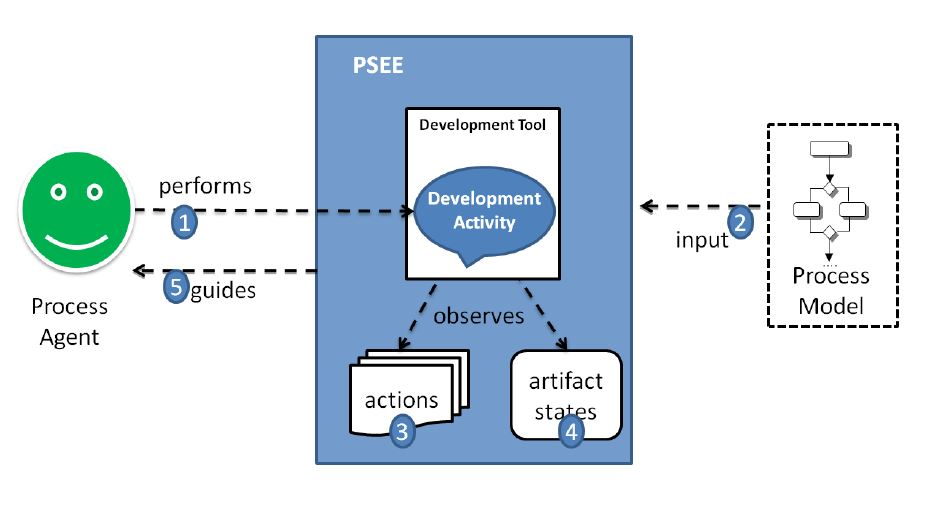
\includegraphics[width=13cm]{role.jpg}
\caption{\label{rolepsee}Rôle d'un PSEE \cite{alm}}
\end{figure}
\clearpage
Le PSEE prend en entrée le modèle de procédé et permet à l'agent de réaliser l'activité de « développement de logiciel ». Dans le but de s'assurer que les activités en cours respectent le modèle de processus définit, le PSEE observe les actions effectuées par les agents. Si les agents ne suivent pas les processus définis, le PSEE doit les guider dans la bonne direction. Le fait d'exécuter une action ne respectant pas les règles décrit dans le modèle de procédé est appelée \textbf{« variation »} ou \textbf{« déviation »}.  
Il existe plusieurs PSEE, mais la plupart ne supportent pas la notion de la gestion de variation dans le processus de développement du logiciel. Dans cette partie, nous allons faire une présentation de certains PSEE et également la manière dont ils gèrent les variations par rapport au prévisionnel.
\subsection*{EPOS}
A décrire
\subsection*{RHODES}
A décrire
\subsection*{SPADE}
A décrire


